\section{Introdução} \bigskip
Nos dias de hoje, o voluntariado é cada vez mais praticado na nossa sociedade. Segundo um estudo realizado pelo INE - Instituto Nacional de Estatística, em 2019, cerca de 6,4\% da população portuguesa realiza trabalho voluntário, uma percentagem que cresceu ligeiramente face aos resultados obtidos em 2012 (5,9\%).$^{\cite{estatistica_2019}}$
\par \bigskip

O trabalho voluntário, ou voluntariado, segundo o diário da república, tem como definição: \par \bigskip

\textit{
	``O conjunto de ações de interesse social e comunitário realizadas de forma desinteressada por pessoas, no âmbito de projetos, programas e outras formas de intervenção ao serviço dos indivíduos, das famílias e da comunidade desenvolvidos sem fins lucrativos por entidades públicas ou privadas.``
}$^{\cite{decreto_lei_71/98}}$ \par \bigskip

Cabe assim ao voluntário (pessoa que realiza o voluntariado) e entidades o papel fulcral na sociedade de tentar enriquecer a mesma sem qualquer contrapartida. \par \bigskip

Para os voluntários, a participação em ações de voluntariado permite a obtenção de competências multi-disciplinares que são valorizadas no mundo profissional, e como tal, cada vez mais empresas dão valor a candidatos que participam nestas ações. \par \bigskip

Atualmente, a candidatura ao voluntariado é efetuada através de múltiplas plataformas, como redes sociais e \textit{websites}, algo que descentraliza estes serviços porque cada organização usa o seu próprio modelo (figura 1).

\bigskip

\begin{figure}[h]
	\centering
	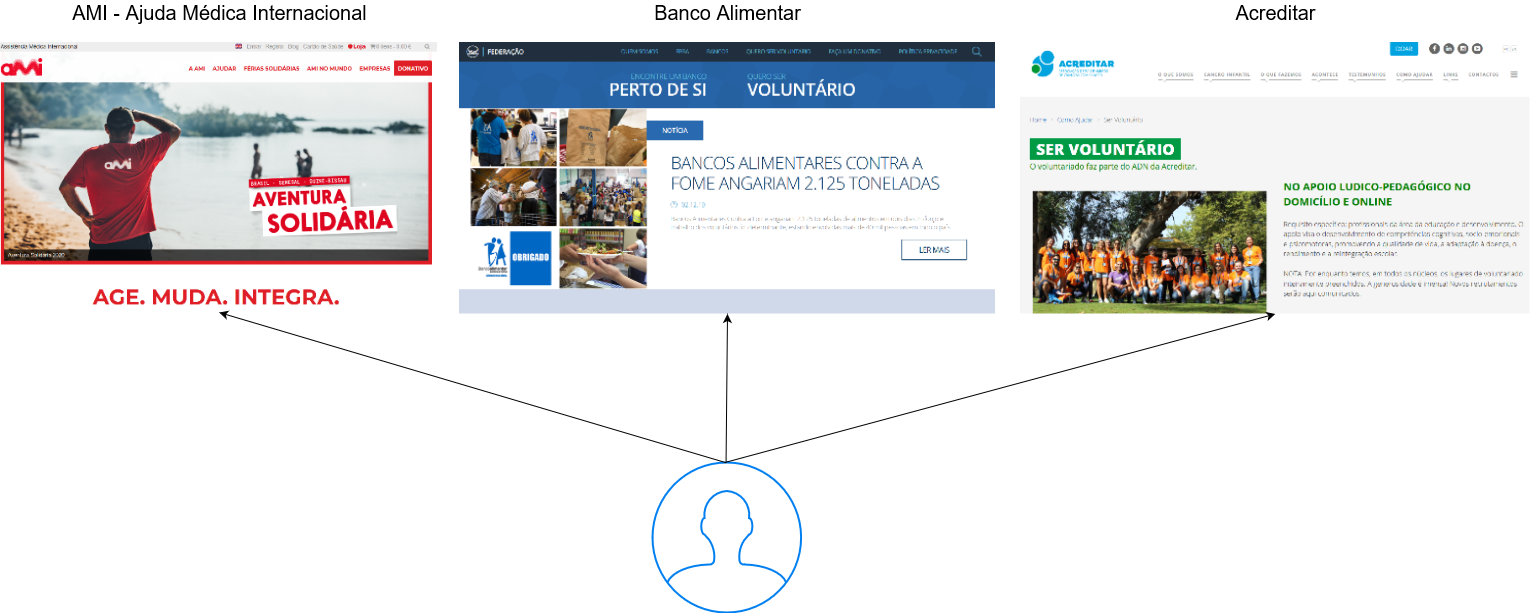
\includegraphics[scale=0.225]{services-decentralized}
	\caption{Modelo descentralizado de divulgação de voluntariado}	
\end{figure}

\newpage

O nosso projeto tem como objetivo desenvolver uma rede social  com foco no voluntariado. A plataforma proposta irá disponibilizar às entidades organizadoras a possibilidade de divulgar e organizar estas ações, e aos voluntários, serviços que facilitam aos mesmos manterem-se informados e participarem nas acções do seu interesse (figura 2).

\bigskip \bigskip \bigskip

\begin{figure}[h]
	\centering
	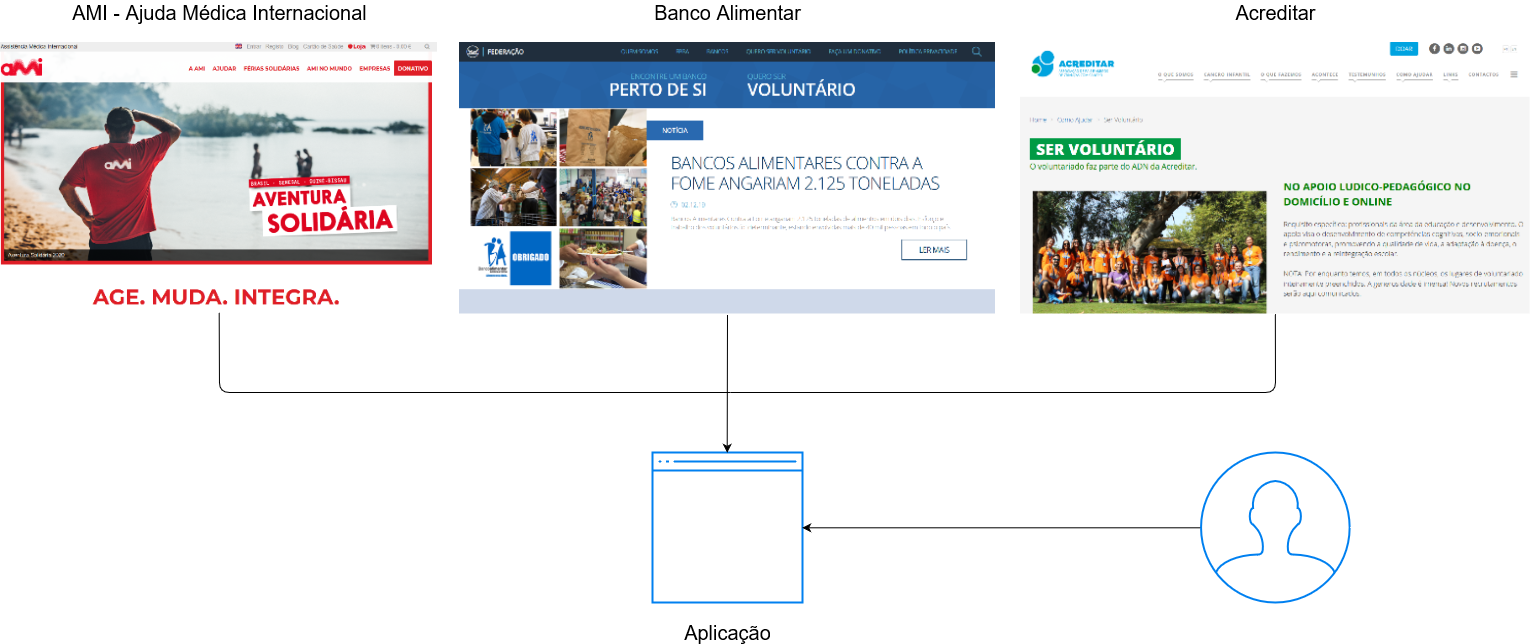
\includegraphics[scale=0.225]{services-centralized}
	\caption{Conceito do projeto}
\end{figure}

\subsection{Organização do relatório}

O presente relatório começará por analisar a problemática atual da divulgação de ações de voluntariado, apresentando de seguida o modelo de arquitetura proposto, mencionando também as soluções e as tecnologias a usar. \par \medskip

Foi desenvolvido um capítulo associado a cada componente do projeto (\textit{web} API, aplicação \textit{mobile} e cliente \textit{browser}), discutindo mais em detalhe as opções tomadas durante o desenvolvimento dos mesmos. \par \medskip

Na fase final do relatório é também discutido o planeamento e desenvolvimento do projeto e as conclusões tiradas durante a evolução do mesmo.
























